\section{Models}



In this study, let us define a model ${h}_{\theta }$ as a function ${h}$  defined on $ \mathbb{N}$, with parameters $\theta$ and trained on the data $\mathcal{D}$.
In the training phase, $\hat{\theta}$,  an estimator of $\theta$ is computed from $\mathcal{D}$, and used for the prediction.  
I deisgned two types of models: the first type correspond to models which are only trained on the time series we want to predict (the number of hospitalized in our case), and the second type of models are trained on the time series we want to predict, but also on other time series that can be relevant to predict the number of hospitalized (the mobility and the number of infected). 
All of these models were implemented in Python, and are available on the github repository provided with this report (\ref{github-link}).
During the training or predicting phase, the computation sometimes fails (for instance, when the matrix is non-inversible for the linear regression model). 
The model then outputs the value of the moving average model (see \ref{sec:moving_average}), which can be interpreted as a naive output when the computation fails. \\[0.3cm]
\textbf{Task of a model}: \\

Each model ${h}$ is given : 

\begin{enumerate}
    \item A training set $\mathcal{D}$
    \item A reach of prediction $r$
    \item A confidence threshold $\alpha$
\end{enumerate}


And outputs: 

\begin{enumerate}
    \item A prediction $\hat{Y}_r$
    \item A $(1-\alpha)$ confidence interval on the prediction, $I_{\alpha, r}$
\end{enumerate}

The model will train on the data $\mathcal{D}$ to compute $\hat{\theta}$ the parameter estimator and the output $\hat{Y}_r = {h}_{\hat{\theta}}(r)$.


\subsection{The SIRH model}



\begin{figure}[h]
    \centering
    \begin{tikzpicture}[
        roundnode/.style={circle, draw=blue!60, fill=gray!5, very thick, minimum size=7mm},
        arrow/.style={-{Stealth[scale=1]}, thick},
        every node/.style={scale=2.0}
        ]

        % Nodes
        \node[roundnode]      (s)                     {S};
        \node[roundnode]      (i) [right=of s]        {I};
        \node[roundnode]      (h) [right=of i]        {H};
        \node[roundnode]      (r) [below=of i]        {R};

        % Arrows
        \draw[arrow] (s) -- (i) node[midway, above, font=\footnotesize] {$\beta$};
        \draw[arrow] (i) -- (h) node[midway, above, font=\footnotesize] {$h$};
        \draw[arrow] (i) -- (r) node[midway, left, font=\footnotesize] {$\gamma_i$};
        \draw[arrow] (h) -- (r) node[midway, right, font=\footnotesize] {$\gamma_h$};

    \end{tikzpicture}
    \caption{Scheme of the SIRH model}
    \label{fig:sirh}

    
\end{figure}

The SIRH model (Fig.\ref{fig:sirh}) is an extension of the classic compartemental SIR (Susceptible-Infectious-Recovered) model used to describe the spread of infectious diseases.
In the SIRH model, a fourth compartment, "H" for "Hospitalized," is added. 
Each compartment corresponds to the number of person in the state of health of the compartment. 
The evolution of the number of person in each compartment is described by a system of ordinary differential equations: 

\begin{equation}
    \label{eq:sirh}
    \left\{
    \begin{aligned}
        &\frac{dS}{dt} = - \beta \frac{SI}{N} \\
        &\frac{dI}{dt} = \beta \frac{SI}{N} - \gamma_i I - h H \\
        &\frac{dR}{dt} = \gamma_i I + \gamma_h h \\
        &\frac{dH}{dt} = h I - \gamma_h H
    \end{aligned}
    \right.
\end{equation}

At $t=0$, the values of $(S_0, I_0, R_0, H_0)$ are fixed to $(10^6 -1, 1, 0, 0,) $. 
As the system of equation can't be directly solved, we use a Euler method to solve it : \\


\begin{equation}
    \left\{
    \begin{aligned}
        S_{t+dt}=S_t + dt \frac{dS}{dt}\\
        I_{t+dt}=I_t + dt \frac{dI}{dt}\\
        R_{t+dt}=R_t + dt \frac{dR}{dt}\\
        H_{t+dt}=H_t + dt \frac{dH}{dt}\\
    \end{aligned}
    \right.
\end{equation}


We chose to fix $dt=0.001$. 


To train this model, we minimize the least squares error between the curve of the number of hospitalized observed to the curve of the number of hospitalized of the training data with respect to $\theta = (\beta, \gamma_i, \gamma_h, h)$. 
I implemented some variations of the model in which $\gamma_i$, $\gamma_h$ or both were fixed to the value $0.2$ (see the Table.\ref{tab:sirh_models_parameters}).
This value of $0.2$ seems arbitrairy but corresponds to an expected value of recovery of 5 days and sometimes helps the curve fir function to converge, as the computations sometimes fails to optimize on the 4 parameters. 

% table 5 x 3 : 

\begin{table}[ht]
\centering
\begin{tabular}{|c|c|c|}
\hline
 &$\gamma_i$ & $\gamma_h$ \\
\hline
SIRH1 & 0.2 & 0.2 \\
\hline
SIRH2 & 0.2 & free \\
\hline
SIRH3 & free & 0.2 \\
\hline
SIRH4 & free & free \\
\hline
\end{tabular}
\caption{Difference between the SIRH models}
\label{tab:sirh_models_parameters}
\end{table}
In the prediction phase, a $r$ day SIRH simulation is launched, with the parameter $\hat{\theta}$ computed during the training phase. 
The initial values for $S$ and $I$ correspond to the last value of the fit of the training phase. 
The initial value for $H$ corresponds to the last value of $\mathcal{D}$, the trainig data. 
The initial value of $R$ is fixed by the previous values as the equation $S_t + I_y + R_t + H_t = N$ is always true. 
The confidence interval of the prediction is computd thanks to a linearization and the use of the delta-method (see \ref{sec:ci})

A SIRH model of the second type was implemented. 
It has the same structure but uses the mobility data and the number of infected to be more precise. 
The idea is the same, but there are two differences : 
\begin{itemize}
    \item $\beta$ varies with the time as a linear combination of the mobility : $\beta_t = a + b \times m_t$ (which is inspired from \cite{gerlee2021predicting})
    \item The data is fitted to both the number of hospitalized and the number of infected. 
\end{itemize}
To write it more formally, let $H_\theta(t)$ and $I_\theta(t)$ be the number of hospitalized and infected at time $t$ in the SIRH model with parameters $\theta$.
Let $Y_{H, t}$ and $Y_{I, t}$ be the number of hospitalized and infected at time $t$ in the data.
We have :\\

$\hat{\theta} = \underset{\theta \in \mathbb{R}^5}{\operatorname{argmin}} \sum_{t=1}^{n} (\frac{H_\theta(t) - Y_{H, t}}{\underset{t \in \{1, ..., n \}}{\operatorname{max(Y_{H, t})}}})^2 + (\frac{I_\theta(t) - Y_{I, t}}{\underset{t \in \{1, ..., n \}}{max(Y_{I, t})}})^2$\\

With $\theta = (a, b, \gamma_i, \gamma_h, h)$ and $m_t$ the mobility at time $t$.
The normalization factors enables to prevent the optimization to focus on the number of infected, which is bigger than the number of hospitalized. 
During my first tries, I hadn't normalized the data and the curve of the infected was almost perfectly fitted to the curve of the SIRH model, but the curve of the hospitalized was flat. 
Once again, a variation of the SIRH model was implemented, in which the value of $\gamma_h$ and $\gamma_i$ is fixed to $0.2$. 
SIRH multi 1 refer to the model in which $\gamma_h$ and $\gamma_i$ are free and SIRH multi 2 refer to the model in which $\gamma_h$ and $\gamma_i$ are fixed to $0.2$.



\subsection{ARIMA and VAR models} 

The ARIMA and VAR models are used for time-series forecasting and have outperformed many models in pandemic forecasting (see \cite{kufel2020arima} and \cite{shang2021regional}).
The $ARIMA(p, d, q)$ model is the sum of an $AR(p)$ and a $MA(q)$ model applied on the time series differenciated $d$ times. 
It follows the equation : \\
$Y_{t}^{d}=\alpha+\sum_{i=1}^{p}\beta_{t-i}\,Y_{t-i}^{d}\,+\,\sum_{j=1}^{q}\phi_{t-j}\,\epsilon_{t-j} \label{eq:arima}$\\ 
where $Y_{t}^{d}$ is the time series at time $t$, $d$ is the order of the differenciation, $\alpha$ is a constant, $p$ is the order of the autoregressive part, $q$ is the order of the moving average part and $\epsilon_{t-j}$ is the difference between the prediction of the model and the real value at time $t-j$.\\
The coefficient are estimated through maximum likelihood estimation. 
This method is implemented in the \texttt{statsmodels} library, which directly provides prediction and confidence intervals.
I realized a grid search on a single pandemic to identify the combination of parameters that would optimize the prediction accuracy. 
I found an optimal value for $p= 3, d=0, q=3$. 

The VAR model is a multi-dimensional $AR$ model, in which different variables are predicted. 
It so corresponds to a second type model. 
This model exploits the correlation between variables and the value of the parameters of a VAR have physical sense as they can be interpreted to find correlations between variables. 
Let $Y_{1,t}, ..., Y_{k,t}$ be the times series (in our case, $k=3$ and they correspond to the number of hospitalized, the number of infected and the mobility data).




\begin{equation*}
\begin{aligned}
VAR(p) : 
\begin{pmatrix}
Y_{1,t} \\
Y_{2,t} \\
\vdots \\
Y_{k,t}
\end{pmatrix}
&=
\begin{pmatrix}
c_1 \\
c_2 \\
\vdots \\
c_k
\end{pmatrix}
+
\begin{pmatrix}
\phi_{11,1} & \phi_{12,1} & \cdots & \phi_{1k,1} \\
\phi_{21,1} & \phi_{22,1} & \cdots & \phi_{2k,1} \\
\vdots & \vdots & \ddots & \vdots \\
\phi_{k1,1} & \phi_{k2,1} & \cdots & \phi_{kk,1}
\end{pmatrix}
\begin{pmatrix}
Y_{1,t-1} \\
Y_{2,t-1} \\
\vdots \\
Y_{k,t-1}
\end{pmatrix} \\
&\quad + \cdots 
+ 
\begin{pmatrix}
\phi_{11,p} & \phi_{12,p} & \cdots & \phi_{1k,p} \\
\phi_{21,p} & \phi_{22,p} & \cdots & \phi_{2k,p} \\
\vdots & \vdots & \ddots & \vdots \\
\phi_{k1,p} & \phi_{k2,p} & \cdots & \phi_{kk,p}
\end{pmatrix}
\begin{pmatrix}
Y_{1,t-p} \\
Y_{2,t-p} \\
\vdots \\
Y_{k,t-p}
\end{pmatrix}
+
\begin{pmatrix}
\epsilon_{1,t} \\
\epsilon_{2,t} \\
\vdots \\
\epsilon_{k,t}
\end{pmatrix}
\end{aligned}
\end{equation*}
    


Again, the $\phi_{i,j,k}$ and  $c_i$ are estimated through maximum likelihood estimation with the \texttt{statsmodel} librairy. 
The confidence intervals are also directy provided by the librairy.



\subsection{The moving average model}
\label{sec:moving_average}

A mere moving average model was also implemented. 
It returns a constant prediction that correspond to the mean of the 7 past days. 
The confidence intervals are computed by assuming that the predictions follow a normal distribution of variance equal to the variance of the 7 last data-points.
This model is used as a baseline, indeed, a model that does not manage to outperform the moving average model would not be useful. 

\subsection{Exponential regression}

An exponential regression model was implemented.
It corresponds to fitting the data of the number of hospitalized ($Y_t$) to the function $E_{a, b, c}(t) = a \times e^{b t} +c$.
The value of $\theta = (a, b, c)$ is computed through a least square minimization method.
The confidence interval on the prediction is estimated with the same method as SIRH (see \ref{sec:ci}). 

An exponential regression of the second type was also implemented: \\
The data of the number of hospitalized is fitted to the function $E_{a, b, c, d, e}(t) = a \times e^{b m_{t-i} + c  t + d \times inf_{t-j} }+e$.\\
$m_t$ is the mobility data at time $t$ and $inf_t$ is the number of infected at time $t$.
The value of $\theta = (a, b, c, d, e)$ is computed through a least square method.
The optimal value of the time lag $i$ and $j$ is optimized during the training phase through a grid search among all the values between 0 and 14. 
The confidence interval on the prediction is estimated with the same method as SIRH (see \ref{sec:ci}). 

\subsection{Machine learning models}
\label{sec:mlmodels}

In order to implement machine learning regressor, I converted the time-series $Y_{t,  t \in \{1, \hdots n\}}$ in a training set $(X_i, Y_i)$ such that : \\
$\forall i \in \{1, ..., n\}, X_i = (Y_{i-1}, Y_{i-2}, ..., Y_{i-20})$.\\

I have then trained and optimized both regressors : the linear and the bayesain regressors, which were the only one that did not output absurd results on the \texttt{scikit-learn} models among : linear regression, bayesian regression, Gradient boosting regressor, Random Forest regressor and SVR. 
The Bayesian ridge model was implemented with the default prior of the \texttt{scikit-learn} librairy (a gamma distribution with shape parameter $10^{-6}$ and scale parameter $10^{-6}$).
The confidence interval for the linear regression prediction was computed as follow : \\
Let us suppose that the data follows a linear regression model : $Y = X\beta + \epsilon$, with $Y \in \mathbb{R}^n$, $X \in \mathbb{R}^{n \times d}$, $\beta \in \mathbb{R}^d$ and $\epsilon \sim \mathcal{N}(0, \sigma^2)$.
The least square estimator of $\beta$ is $\hat{\beta} = (X^T X)^{-1} X^T Y$.
If we have new data $\tilde{X} \in \mathbb{R}^{1 \times d}$ that we want to predict, the prediction is  : \\

$
\begin{aligned}
    \tilde{Y} & = \tilde{X} \hat{\beta} \\
    &  = \tilde{X} \hat{\beta} = \tilde{X} (X^T X)^{-1} X^T Y \\
    &  = \tilde{X} (X^T X)^{-1} X^T (X\beta + \epsilon) \\
    &  = \tilde{X} \beta + \tilde{X} (X^T X)^{-1} X^T \epsilon.\\
\end{aligned}
$
\newline
$\tilde{Y}$ follows a normal distribution of expected value $\tilde{X} \beta$ and variance $\tilde{X} (X^T X)^{-1} \tilde{X}^T \sigma ^2$.\\
The confidence interval on bayesian regression was directly computed with the variance of the parameters given by the scikit-learn librairy and the delta method. 

\subsection{Ensemble model}

It has been showned (see \cite{cramer2022evaluation} and \cite{reich2019accuracy}), that ensemble models, which combine the outputs of many models, can outperform by far individual models.
I have implemented an ensemble model which is a linear combination of the outputs of the 13 models described above, with the exponential models removed.
The weights of this model were found my minimizing the least-squared error between the prediction of the ensemble model and the real value of the number of hospitalized on a train set of approximately 80\% of the pandemic generated. 
They are represented in the Fig.\ref{fig:ensemble_weights}.
As the ensemble model only outputs a single value without confidence intervals, it is only evaluated with the RMSE metric. 
\begin{figure}
    \centering
    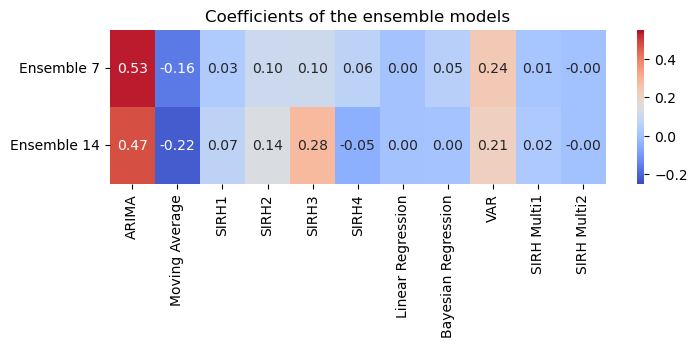
\includegraphics[width=0.5\textwidth]{figures/esb_coefs.png}
    \caption{Weights of the ensemble models}
    \label{fig:ensemble_weights}
\end{figure}
\subsection{Computing confidence intervals on the prediction}
\label{sec:ci}
In this section, we prove the formula used for in the code to compute the confidence intervals. 
The following proof is inspired from \cite{ruckstuhl2010introduction} and \cite{powellasymptoticsforleastsquares}. 
I have assembled individuals proofs from these two articles to get the final results. 
Some notations and steps are identical to what we can find in the paper and are explicitely cited. 
This problem is a non linear regression problem. 
The proof is made of three steps. 
First, we linearize the problem around the solution to get back to a linear regression problem. 
Then, we show that the estimator of the linear regression problem is asymptotically normal.
Finally, we use the delta-method to obtain the asymptotic normality of the non linear regression estimator . \\


\textbf{Assumption}:
\\[0.5cm]
We suppose that the data of the pandemic observed follows the model $h$, of parameter $\theta^* \in \mathbb{R}^d$. Let $Y_i$, $ i = 1, \ldots, n$ be the number of hospitalized at each day. We suppose that: $Y_i = h_{\theta ^* } (i) + \epsilon_i$, with $\epsilon_i \sim \mathcal{N}(0, \sigma^2)$, iid, and independent from all the other variables. The objective is to estimate $\theta^*$. We use $\hat{\theta}$, the least square estimator of $\theta^*$ as an estimator of $\theta^* $:
\[
\hat{\theta} =  \underset{\theta \in \mathbb{R}^d}{\operatorname{argmin}} \sum_{i=1}^{n} (Y_i - h_{\theta}(i))^2
\]
This problem is a non-linear regression problem on the regressors $i$. 
We also suppose that $h_\theta$ is differentiable.
Finally, we suppose that 
\begin{equation}
\exists A_0 \in \mathbb{R} ^{1 \times d},  \frac{1}{n} \sum_{i=1}^{n} \nabla_\theta h_{\theta^*}(i) \nabla_\theta h_{\theta^*}(i)^T \underset{n \rightarrow +\infty }{\rightarrow}  A_0^T A_0 .\label{hyp:major}  \\
\end{equation}

\textbf{STEP 1 :}\\
\label{step:step1}

Let:
\begin{align*}
Y &= \begin{pmatrix}
Y_1 \\
\vdots \\
Y_n
\end{pmatrix} \\
h_\theta &= \begin{pmatrix}
h_\theta(1) \\
\vdots \\
h_\theta(n)
\end{pmatrix}
\end{align*}

We have:
\[
\hat{\theta} =  \underset{\theta \in \mathbb{R}^d}{\operatorname{argmin}}  \left\lVert Y - h_\theta \right\rVert ^2
\]

Now, if $\theta$ is close enough to $\theta^*$, we can write (from \cite{ruckstuhl2010introduction}):
\[
\forall i \in \{ 1, ..., n\} :  h_\theta(i) = h_{\theta^*} (i ) + (\theta - \theta^*)^T\nabla_\theta h_{\theta^*}(i) 
\]
which leads to:
\[
\hat{\theta} =  \underset{\theta \in \mathbb{R}^d}{\operatorname{argmin}}  \left\lVert Y - h_{\theta^*}  - (\theta - \theta^*)^T\nabla_\theta h_{\theta^*}\right\rVert ^2
\]

Let us define (from \cite{ruckstuhl2010introduction}): \\
\begin{align*}
\tilde{Y} &= Y - h_{\theta^*} \\
\beta &= \theta - \theta^* \\
\hat{\beta} &= \theta - \hat{\theta}
\end{align*}

and let us define the matrix $A \in \mathbb{R} ^{n \times d }$ such that $\forall i \in \{ 1, ..., n\}, \forall j \in \{1, ..., d\}, A_{i, j} = \frac{dh_{\theta^*}}{d\theta_j}(i)$.
(\cite{ruckstuhl2010introduction})

The previous problem can be re-written as:
\[
\hat{\beta} =  \underset{\beta \in \mathbb{R}^d}{\operatorname{argmin}}  \left\lVert \tilde{Y} - A \beta \right\rVert ^2
\]

This is now a  linear regression problem on the regressors $\nabla_\theta h_{\theta^*}(i)$.



\textbf{STEP 2 :}\\
\label{step:step2}



Let us solve this problem in the general case.

Let $(A_i, \tilde{Y_i})$ be the observations.
In our case, $A_i = (\nabla_\theta h_{\theta*} (i))^T$, the rows of $A$,  and is a fixed quantity.  
Let us assume that $\tilde{Y_i} = A_i \beta ^* + \epsilon'_i $, with $\epsilon'_i \sim \mathcal{N}(0, \sigma'^2)$.

The solution of this problem is explicitly (from \cite*{powellasymptoticsforleastsquares}):
\[
\hat{\beta } = (A^T A ) ^{-1} A^T \tilde{Y}
\]

This least-square estimator is unbiased:
\[
\mathbb{E}[\hat{\beta}] = \beta^*
\]


\[
\hat {\beta } = \left(  \sum_{i=1}^{n}   A_i ^T A_i \right) ^{-1}    \times \left(  \sum_{i=1}^{n} A_i ^T \tilde{Y_i } \right)
\]

\[
\hat {\beta } =\frac{n}{n} \left(  \sum_{i=1}^{n}   A_i ^T A_i \right) ^{-1}    \times \left(  \sum_{i=1}^{n} A_i ^T \tilde{Y_i } \right)
\]

\[
\hat {\beta } = \left( \frac{1}{n} \sum_{i=1}^{n}   A_i ^T A_i \right) ^{-1}    \times \left( \frac{1}{n} \sum_{i=1}^{n} A_i ^T \tilde{Y_i } \right)
\]

Let us denote, with the notations from \cite{powellasymptoticsforleastsquares}:
\[
\hat{D}  = \frac{1}{n} \sum_{i=1}^{n}   A_i ^T A_i , \quad \text{and} \quad \hat{\delta}  = \left( \frac{1}{n} \sum_{i=1}^{n} A_i ^T \tilde{Y_i } \right)
\]

We have:
\[
\hat{\beta} = \hat{D} ^{-1} \hat{\delta}
\]

\[
\hat{D}  \underset{a.s}{\rightarrow} D \text{,  with } D = \mathbb{E}[A_i^T A_i ] = A_0^T A_0 \text{ (cf Hyp \ref{hyp:major})}
\]
$\hat{\delta}$ is the empirical mean of random variables independant but non identically distributed. 
We therefore cannot use the Kolmogorov's Strong Law of Large Numbers. 
There exists a law of large number for independant and non identically distributed random variables, which assesses that (see Therom 12 from \cite{suquet2004lois}):




\theoremstyle{plain}
\newtheorem{theorem}{Theorem}

\begin{theorem}
    \label{thm:1}
    Let $(X_k)$ be a sequence of independent random variables such that:
    \begin{enumerate}
        \item For all $k \geq 1$, $\mathbb{E}(X_k^2) < +\infty$;
        \item There exists an increasing sequence $(a_k)$ of strictly positive real numbers tending to infinity, such that
        \[
        \sum_{k=1}^{+\infty} \frac{\mathrm{Var}(X_k)}{a_k^2} < +\infty.
        \]
    \end{enumerate}
    Then, $\frac{S_n - \mathbb{E}S_n}{a_n}$ converges almost surely to $0$. If additionally $a_n^{-1} \mathbb{E}S_n \to m$, then $\frac{S_n}{a_n}$ converges almost surely to $m$.\\[2cm]
\end{theorem}

Let $ i \in \{1, ..., n\}$.\\[0.2cm]
$X_i = A_i ^T \tilde{Y_i} = A_i^T A_i \beta^* + A_i ^T \epsilon'_i$. \\
The random values $X_i$ are independant random variables.\\
$\forall i \in \{ 1, ...  n \}, \mathbb{E}[X_i^2] = \mathbb{E}[X_i] ^2 + A_0 ^T A_0 \sigma'^2 < + \infty $.\\

$\sum_{i=1}^{\infty } \frac{Var(X_i)}{i^2} = \sum_{i=1}^{\infty } \frac{A_0^T A_0 \sigma'^2}{i^2} =  A_0^T A_0 \sigma'^2 \sum_{i=1}^{\infty } \frac{1}{i^2} < + \infty$.\\

Moreover,  $\frac{1}{n} \sum_{i=1}^{n} \mathbb{E}[X_i] =\frac{1}{n} \sum_{i=1}^{n} A_i^T A_i \beta^* = \frac{\beta^*}{n} \sum_{i=1}^{n} A_i^T A_i \underset{n\rightarrow \infty}{\rightarrow} \beta ^*  A_0 ^T A_0 $ (see \ref{hyp:major}).\\

Therefore, with Theorem \ref{thm:1}, we have :  $\frac{1}{n} \sum_{i=1}^{n} A_i ^T \tilde{Y_i} \underset{a.s}{\rightarrow}  \beta ^*  A_0 ^T A_0 $

\[
\hat{\delta}   \underset{a.s}{\rightarrow}  \delta = A_0 ^T A_0 \beta^*
\] 

$ \hat{\beta} = \hat{D}^{-1} \hat{\delta}  \underset{a.s}{\rightarrow}  D^{-1} \delta $ , as the following function $\phi$ is continuous:
\[
\phi: \left\{
\begin{array}{rcl}
\mathcal{GL}_n(\mathbb{R}) & \to & \mathcal{GL}_n(\mathbb{R}) \\
M & \mapsto & M^{-1}
\end{array}
\right.
\]


Now, let us show that $\hat{\beta}$ is asymptotically normal (proof from \cite{powellasymptoticsforleastsquares}): 

\begin{align*}
    \sqrt{n} ( \hat{\beta} - \beta ^* ) &= \sqrt{n} (\hat{D}^{-1} \hat{\delta} - \beta ^* ) \\
     &= \sqrt{n} (\hat{D}^{-1} \hat{\delta} - \hat{D}^{-1} \hat{D} \beta ^* ) \\
     &= \sqrt{n} \hat{D}^{-1} (\hat{\delta} -  \hat{D} \beta ^* )  \\
     &= \sqrt{n} \hat{D}^{-1} \left( \frac{1}{n} \sum_{i=1}^{n} A_i ^T \tilde{Y_i} - \frac{1}{n}  \sum_{i=1}^{n}  A_i ^T A_i \beta ^* \right)  \\
     &= \frac{\sqrt{n}}{n} \hat{D}^{-1} \left( \sum_{i=1}^{n} A_i ^T (\tilde{Y_i} -    A_i \beta ^* ) \right)   \\
     &= \frac{1}{\sqrt{n}}  \hat{D} ^{-1} \left( \sum_{i=1}^{n}  A_i ^T \epsilon _ i \right)  
\end{align*}

This line is made of two terms. Let's show that each one of them converges in law. 

\begin{align*}
    \frac{1}{\sqrt{n}} \left( \sum_{i=1}^{n}  A_i^T \epsilon'_i \right) &= \sqrt{n} \left( \frac{1}{n} \sum_{i=1}^{n}  A_i^T \epsilon'_i \right) \\
    &= \sqrt{n} \left( \frac{1}{n} \sum_{i=1}^{n}  A_i^T \epsilon'_i - 0 \right) \\
    &\xrightarrow{\mathcal{L}} \mathcal{N}(0, \text{Var}(A_i^T \epsilon_i) )
\end{align*}


Yet, as $\epsilon_i $ and $  A_i $ are independant, and $\mathbb{E} [ A_i^T \epsilon'_i] = 0 $ , $\text{Var}(A_i^T \epsilon_i) = \mathbb{E}[A_i ^T A_i \epsilon_i ^2 ] = \mathbb{E} [ A_i ^T A_i ] \sigma'^2 =A_0^T A_0 \sigma'^2  $. 

Finally, $\frac{1}{\sqrt{n}} \left( \sum_{i=1}^{n}  A_i^T \epsilon'_i \right) \xrightarrow{\mathcal{L}} \mathcal{N}(0, D \sigma'^{2})$. 

On the other hand, $\hat{D}^{-1} \xrightarrow{\mathcal{L}} D^{-1} $, which is constant.

Finally, with Slutsky, we obtain that: 

\begin{align*}
    \sqrt{n} (\hat{\beta} - \beta^*) &\xrightarrow{\mathcal{L}} D^{-1}\mathcal{N}(0, D \sigma'^2) \\
    &\xrightarrow{\mathcal{L}} \mathcal{N}(0, D^{-1} (D \sigma'^2) (D^{-1})^T) \\
    &\xrightarrow{\mathcal{L}} \mathcal{N}(0, D^{-1} D \sigma'^2 (D^{-1})^{T}) \\
    &\xrightarrow{\mathcal{L}} \mathcal{N}(0, \sigma'^2 D^{-1}) \\
    &\xrightarrow{\mathcal{L}} \mathcal{N}(0, \sigma'^2 (A_0^T A_0)^{-1})
\end{align*}


Let's get back to the first problem: 

As $\beta ^* = 0 $ and $\hat{\beta} = \hat{\theta} - \theta ^* $, we have: 

\[
\sqrt{n} (\hat{\theta} - \theta^*) \xrightarrow{\mathcal{L}} \mathcal{N}(0, \sigma^2 (A_0^T A_0)^{-1})
\]

and, 
\[
\hat{\theta} \sim \mathcal{N}(\theta^*, \frac{\sigma^2}{n} (A_0^T A_0)^{-1})
\]

As a partial conclusion, we have that $\hat{\theta}$ is asymptotically normal.



\textbf{STEP 3 :}\\
\label{step:step3}


Let $\Sigma$ be the covariance matrix estimated from the computation of $\hat{\theta}$. 

As $\hat{\theta}$ is asymptotically normal, we can apply the delta-method: 

\[
\sqrt{n} (\hat{\theta} -\theta^*) \xrightarrow{\mathcal{L}} \mathcal{N}(0, \ \Sigma)
\]
\[
\sqrt{n} (h_{\hat{\theta}} -h_{\theta^*}) \xrightarrow{\mathcal{L}} \mathcal{N}(0, \nabla_\theta h_\theta ^T \Sigma  \nabla_\theta h_\theta)
\]

And finally: 
\[
h_{\hat{\theta}} \rightarrow \mathcal{N}(h_{\theta^*}, \frac{1}{n}\nabla_\theta h_\theta ^T \Sigma  \nabla_\theta h_\theta)
\]

By estimating $\frac{1}{n} \Sigma$ from \texttt{curve\_fit}, we can compute the confidence interval of the prediction with the quantiles of the normal distribution.
The gradient of $h_\theta$ is approximated through numerical approximation: \\
$\nabla_\theta h_\theta [i] \simeq \frac{h_{\theta + d \theta _ i  } - h_\theta}{dt}$, with $dt=0.0001$. \\

\begin{align*}
    d\theta_i &= \begin{pmatrix}
    \theta_0 \\
    \theta_1\\
    \vdots \\
    \theta_{i-1}\\
    \theta_i + dt \\
    \theta_{i+1}\\
    \vdots \\
    \theta_n 
    \end{pmatrix} \\    
\end{align*}